\section{Pruning Rules}
Grid maps are highy regular problem domains. 
In particular, each node in the grid has a small number of neighbours (usually
8 though some nodes may have less) and each
neighbour is always located in the same position relative to the current node.
We exploit this regularity in order to develop pruning rules that speed up 
individual node expansion operations.
Our goal is to identify and discard neighbours
which do not need to be evaluated in order to reach the goal optimally.
We distinguish between two different sets of rules, depending on whether the 
transition from the current node to its parent involves a straight move or a
diagonal move.

\subsection{Rules For Straight Moves}
\label{sec:prunestraight}
Consider Figure \ref{fig:pruningrules}(a) and (b), in which an arbitrary search
algorithm is expanding a node $x$ by making a straight move from a parent node
$p(x)$ = 4.  In the case of Figure \ref{fig:pruningrules}(a), $x$ is not adjacent to
any obstacle and we can immediately prune the following neighbours:

\begin{enumerate}

\item Neighbour 4. This move has a cost of $c + 1$. However, $p(x)$ was already expanded
with cost $c - 1$.

\item Neighbour 1 (6). This move has a cost of $c  + \sqrt2$ yet the same neighbour
can be reached with cost $c$ from $p(x)$.

\item Neighbour 2 (7). This move has a cost of $c + 1$ yet the same neighbour  can
be reached from $p(x)$ with cost $(c - 1) + \sqrt2$.

\item Neighbour 3 (8). This move has a cost of $c + \sqrt2$ but is symmetric to an
alternative path which passes through $p(x)$ and mentions neighbour 2 (8) but
not $x$.

\end{enumerate}

\noindent In the best case we eliminate 7 of the possible 8 neighbours, leaving
only neighbour 5 to be evaluated.  The worst case is shown in Figure
\ref{fig:pruningrules}(b) and occurs when both neighbours 2 and 7 are blocked; 
since we cannot apply the final pruning rule, the evaluation of neighbours 3 and
8 is forced.
\par
Note that in this example $p(x)$ = 4. Analogous rules 
exist for cases where $p(x)$ is equal to neighbours 2, 5 or 7. We omit these for 
brevity.

\subsection{Rules for Diagonal Moves}
\label{sec:prunediagonal}
 In Figure \ref{fig:pruningrules}(c) and
(d) the search algorithm expands node $x$ by making a diagonal move from the
parent node $p(x)$ = 6.  In the case of Figure \ref{fig:pruningrules}(c) $x$ is
not adjacent to any obstacle and we can immediately prune the following
neighbours:

\begin{enumerate}

\item Neighbour 6. This move has a cost of $c + \sqrt2$. However, $p(x)$ was
already expanded with cost $c - \sqrt2$.

\item Neighbour 4 (7). This moves has a cost $c + 1$ yet the same neighbour can
be reached with cost $(c - \sqrt2) + 1$ from $p(x)$.

\item Neighbour 1 (8). This move has a cost $c + \sqrt2$ yet the same neighbour
can be reached with cost $(c - \sqrt2) + 2$ via an alternative path, which
passes through $p(x)$ and mentions neighbour 4 (7) but not $x$.

\end{enumerate}

\noindent In the best case we eliminate 5 of the possible 8 neighbours, leaving
only neighbours 2, 3 and 5 to be evaluated.  The worst case is shown in Figure
\ref{fig:pruningrules}(d) and occurs when neighbour 4 (7) is blocked. Since we
cannot apply the final pruning rule, the evaluation of neighbour 1 (8) is
forced.  We do not consider the case where both neighbours 4 and 7 are
simultaneously blocked as such moves are impossible and thus disallowed.

As before, we omit analogous rules for the cases where $p(x)$ is equal to
neighbours 1, 3 or 8.

\begin{figure}[tb]
       \begin{center}
		   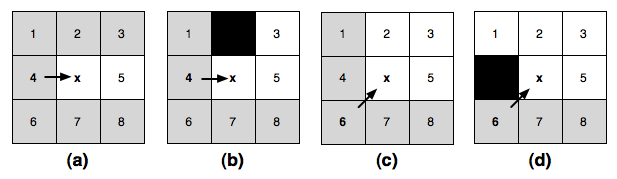
\includegraphics[scale=0.4, trim = 10mm 10mm 10mm 0mm]{diagrams/pruningrules.png}
       \end{center}
	\vspace{-3pt}
       \caption{We show several cases where a node $x$ is reached from its
parent $p(x)$ by either a straight or diagonal move. When $x$ is expanded we can prune from consideration all nodes marked gray.}
       \label{fig:pruningrules}
\end{figure}


\subsection{Optimality}
In the following theorem we prove that searching with the pruning rules
developed thus far has no effect on the completeness or optimality of returned 
solutions. We will show this is true by means of an inductive
argument over the cost associated with any expanded node, often called its 
$g$-value. 

\begin{theorem}
\label{thm:pruningoptimality}
The $g$-value of each node expanded during search is the same 
with or without the application of straight and diagonal node pruning.
\end{theorem}
\begin{proof}
Let $n$ be a node selected for expansion during an arbitrary
optimality-preserving search process which is using straight and diagonal
node pruning. We will show by induction that $g(n)$ must be optimal.
\par
\emph{Basis case: } $n$ is the start node and $g(n) = 0$. No pruning has
occured so this value must be optimal.
\par
\emph{Inductive case: }
Choose $n$ as any node expanded before the completion
of the search. For a contradiction, suppose that $g(n)$ is not optimal.
This can only have occured if $n$ was pruned during the earlier 
expansion of an alternative parent node $x$ s.t. $(x, n)$ never appears on 
the optimal path.
There are two ways to prune $n$ during the expansion of $x$, depending on whether 
$x$ is reached by way of a straight move or a diagonal move.
We know from Sections \ref{sec:prunestraight} and \ref{sec:prunediagonal} 
that in either case if $n$ is pruned the edge $(x, n)$ is either provably
sub-optimal or belongs to a path comprising the nodes 
$\lbrace p(x), x, n \rbrace$ which is symmetric to an alternative path of the same 
length that only mentions the nodes $\lbrace p(x), p(n), n\rbrace$.
Both possibilities contradict the supposition that $g(n)$ is sub-optimal. 
\end{proof}

% \begin{corollary}
%The number of nodes expanded is the same, with or without the application of 
%straight and diagonal node pruning.
%\end{corollary}
%\begin{proof}
%By Theorem \ref{thm:pruningoptimality}, we only prune neighbours which could
%not be improved. 
%\end{proof}
%
